\documentclass[a4paper,14pt]{extarticle}

\usepackage[utf8x]{inputenc}
\usepackage[T1]{fontenc}
\usepackage[russian]{babel}
\usepackage{hyperref}
\usepackage{indentfirst}
\usepackage{here}
\usepackage{array}
\usepackage{graphicx}
\usepackage{caption}
\usepackage{subcaption}
\usepackage{chngcntr}
\usepackage{amsmath}
\usepackage{amssymb}
\usepackage[left=2cm,right=2cm,top=2cm,bottom=2cm,bindingoffset=0cm]{geometry}
\usepackage{multicol}
\usepackage{multirow}
\usepackage{titlesec}
\usepackage{listings}
\usepackage{color}
\usepackage{enumitem}
\usepackage{cmap}
\usepackage{url}

\definecolor{green}{rgb}{0,0.6,0}
\definecolor{gray}{rgb}{0.5,0.5,0.5}
\definecolor{purple}{rgb}{0.58,0,0.82}

\lstdefinelanguage{none}{}

\lstset{
	language={Python},
	backgroundcolor=\color{white},
	commentstyle=\color{green},
	keywordstyle=\color{blue},
	numberstyle=\color{gray}\scriptsize\ttfamily,
	stringstyle=\color{purple},
	basicstyle=\lst@ifdisplaystyle\footnotesize\fi\ttfamily,
	breakatwhitespace=false,
	breaklines=true,
	captionpos=b,
	keepspaces=true,
	numbers=left,
	numbersep=5pt,
	showspaces=false,
	showstringspaces=false,
	showtabs=false,
	tabsize=4,
	frame=single,
	morekeywords={},
	deletekeywords={},
	extendedchars=false,
	columns=fullflexible,
	literate=%
		{~}{{\raise.25ex\hbox{$\mathtt{\sim}$}}}{1}%
		{-}{-}{1}
}

\titleformat*{\section}{\large\bfseries}
\titleformat*{\subsection}{\normalsize\bfseries}
\titleformat*{\subsubsection}{\normalsize\bfseries}
\titleformat*{\paragraph}{\normalsize\bfseries}
\titleformat*{\subparagraph}{\normalsize\bfseries}

\counterwithin{figure}{section}
\counterwithin{equation}{section}
\counterwithin{table}{section}
\newcommand{\sign}[1][5cm]{\makebox[#1]{\hrulefill}}
\newcommand{\equipollence}{\quad\Leftrightarrow\quad}
\newcommand{\no}[1]{\overline{#1}}
\newcommand{\code}[1]{\lstinline[language=none]|#1|}
\graphicspath{{../pics/}}
\captionsetup{justification=centering,margin=1cm}
\def\arraystretch{1.3}
\setlength\parindent{5ex}
\titlelabel{\thetitle.\quad}

\setitemize{topsep=0em, itemsep=0em}
\setenumerate{topsep=0em, itemsep=0em}


\begin{document}

\begin{titlepage}
\begin{center}
	Санкт-Петербургский Политехнический Университет Петра Великого\\[0.3cm]
	Институт компьютерных наук и технологий \\[0.3cm]
	Кафедра компьютерных систем и программных технологий\\[4cm]

	\textbf{ОТЧЕТ}\\
	\textbf{по лабораторной работе}\\[0.5cm]
	\textbf{<<Поиск векторов смещения>>}\\[0.1cm]
	Разработка графических приложений\\[3.0cm]
\end{center}

\begin{flushright}
	\begin{minipage}{0.5\textwidth}
		\textbf{Работу выполнил студент}\\[3mm]
		гр. 3540901/91502 \hfill \sign[1.1cm] \hfill Дьячков В.В.\\[5mm]
		\textbf{Работу принял преподаватель}\\[5mm]
		\sign[5cm] \hfill Абрамов Н.А. \\[5mm]
	\end{minipage}
\end{flushright}

\vfill

\begin{center}
	Санкт-Петербург\\[0.3cm]
	\the\year
\end{center}
\end{titlepage}

\addtocounter{page}{1}


\tableofcontents
\newpage

\section{Программа работы}

Реализовать алгоритмы поиска векторов смещения:

\begin{enumerate}
	\item алгоритм полного перебора;
	\item алгоритм ромбовидного поиска.
\end{enumerate}

\section{Выполнение работы}

\subsection{Вспомогательные функции}

\paragraph{Сравнение изображений}

Для сравнения получаемых изображений будем использовать сумму абсолютных разностей (sum of absolute differences, SAD). Для этого сложим разницу между соответствующими пикселями двух изображений.

\begin{lstlisting}[caption={Фунукция для сравнения изображений}]
def sad(a, b):
	return np.sum(np.abs(a.astype(np.float64) - b.astype(np.float64)))
\end{lstlisting}

\paragraph{Отображение векторов смещения}

Для отображения векторов смещения была реализована функция, принимающая изображение и матрицу смещений. Если для некоторого пикселя определяется смещение, то из него рисуется стрелка при помощи функции \code{cv.arrowedLine}.

\begin{lstlisting}[caption={Фунукция для сравнения изображений}]
def with_arrows(image, moves, block):
	h, w, _ = moves.shape
	motions = cv.cvtColor(image, cv.COLOR_GRAY2RGB)
	block_half = block // 2
	for x in range(h):
		for y in range(w):
			dx, dy = moves[x, y]
			if dx != 0 or dy != 0:
				start = (y * block + block_half, x * block + block_half)
				end = (y * block + dy + block_half, x * block + dx + block_half)
				cv.arrowedLine(motions, start, end, (255, 0, 0))
	return motions
\end{lstlisting}

\subsection{Алгоритм полного перебора}

Алгоритм полного перебора базируется на сравнении исходного
блока со всеми блоками в окне поиска, размер которого устанавливается вручную. Этот метод наиболее вычислительно затратный, но при этом показывает наиболее точные результаты.

\begin{lstlisting}[caption={Поиск векторов смещения при помощи полного перебора}]
def full_search(source, shift, block=16, window=32):
	h, w = source.shape
	moves = np.zeros(shape=(h // block, w // block, 2), dtype=np.int64)
	for i in range(0, h - window - block, block):
		for j in range(0, w - window - block, block):
			source_block = source[i : i + block, j : j + block]
			s_min, k_min, l_min = -1, 0, 0  
			for k in range(window):
				for l in range(window):
					shift_block = shift[k + i : k + i + block, l + j : l + j + block]
					s = sad(source_block, shift_block)
					if (s < s_min or s_min == -1
						or s * 0.9 < s_min and k + l < k_min + l_min):
						s_min, k_min, l_min = s, k, l
		moves[i // block][j // block][0] = k_min
		moves[i // block][j // block][1] = l_min
	return moves
\end{lstlisting}

Подобный метод ожидаемо медленный, так как происходят вычисления, которых можно было бы избежать. Идея реализации заключается в том, что для заданной точки берётся блок с исходного изображения, далее для каждой точки на модифицированном изображении в области поиска высчитывается метрика различия с исходным блоком. Направление в сторону блока с наименьшей разницей метрики и есть направление смещения.

Применим алгоритм к монотонному изображению круга и градиентному изображению квадрата.

\begin{figure}[H]
	\centering
	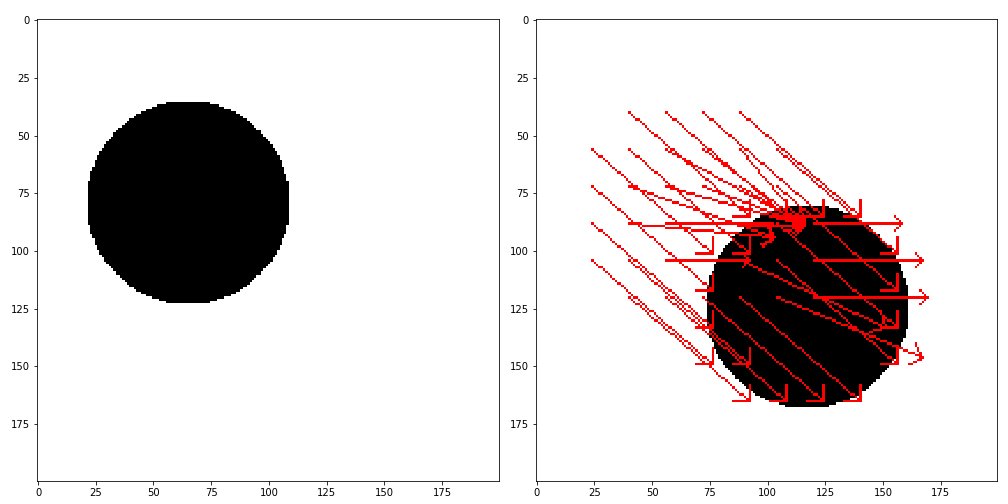
\includegraphics[width=\linewidth]{circle_full}
	\caption{Поиск векторов смещения при помощи полного перебора для монотонного изображения (3 секунды)}
\end{figure}

\begin{figure}[H]
	\centering
	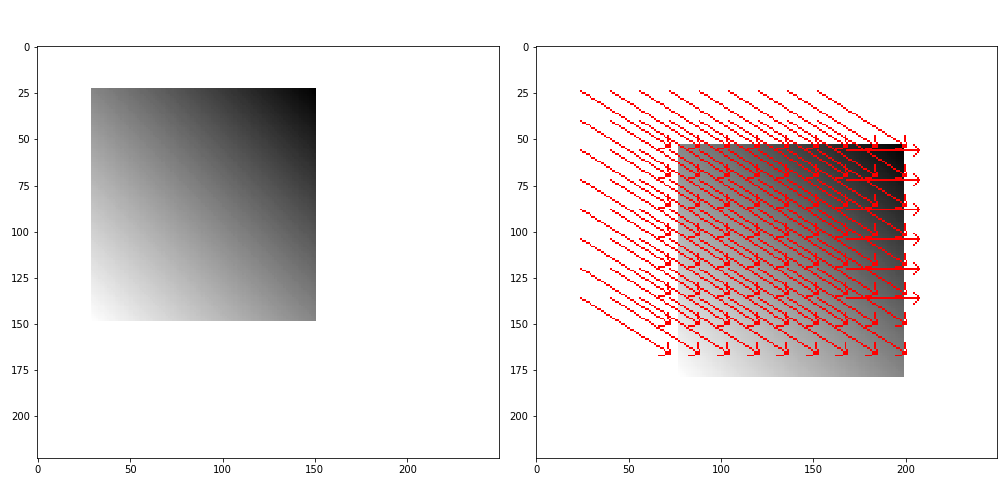
\includegraphics[width=\linewidth]{square_full}
	\caption{Поиск векторов смещения при помощи полного перебора для градиентного изображения (5.3 секунды)}
\end{figure}

Из результатов видно, что несмотря на долгое время работы, вектора смещения определены верно.

\subsection{Алгоритм ромбовидного поиска}

В алгоритме ромбовидного (алмазного) поиска используются два разных фиксированных шаблона:

\begin{itemize}
	\item Большой алмазный шаблон поиска (LDSP);
	\item Шаблон поиска небольших алмазов (SDSP).
\end{itemize}

Чтобы сократить время поиска наименьшего отличающегося блока, поиск будет проводиться не по всем значениям, а лишь по тем, которые находятся в точках ромба. Поиск делится на два этапа: поиск и <<допоиск>>. Этапы отличаются лишь размерами робма, который используется при поиске. Идея ромбовидного поиска заключается в том, что на каждом шаге вычисляются метрики различия для точек ромба, исключая те точки, которые уже были посчитаны на предыдущих шагах. После этого определяется наименьшее значение и шаг повторяется снова, но уже со смещенным центром ромба в точку с минимальным значением метрики.

\begin{lstlisting}[caption={Фунукция для применения билатерального фильтра}]
def diamond_search(source, shift, block=16, window=32):
    def sad_point(source_block, shift, k, l):
        shift_block = shift[k : k + block, l : l + block]
        return sad(source_block, shift_block)

    h, w = source.shape
    window_half = window // 2
    motions = np.zeros(shape=(h // block, w // block, 2), dtype=np.int64)
    diamond_direction_ldsp = [
        [ 0, 0], [ 0, 2], [ 1, 1],
        [ 2, 0], [ 1,-1], [ 0,-2],
        [-1,-1], [-2, 0], [-1, 1]]
    diamond_direction_sdsp = [
        [ 0, 0] ,[ 0, 1] ,[ 1, 0],
        [ 0,-1], [-1, 0], [ 0, 0]]
    
    for i in range(window_half, h - (window_half + block), block):
        for j in range(window_half, w - (window_half + block), block):
            source_block = source[i : i + block, j : j + block]
            sad_space = np.full((window, window), np.inf)
            
            def calculate_dsp(k_center, l_center, diamond_array):
                if (k_center > window_half
                    or k_center < -window_half
                    or l_center > window_half
                    or l_center < -window_half): 
                    return (k_center, l_center)

                sad_local_min = sad_space[k_center, l_center]
                k_local_min = k_center
                l_local_min = l_center
                for (dk, dl) in diamond_array:
                    if sad_space[k_center + dk, l_center + dl] == np.inf:
                        sad_step = sad_point(source_block, shift, k_center + i + dk, l_center + j + dl)
                        sad_space[k_center + dk, l_center + dl] = sad_step
                        if sad_step < sad_local_min:
                            sad_local_min = sad_step
                            k_local_min = k_center + dk
                            l_local_min = l_center + dl
                return (k_local_min, l_local_min)
        
            dk, dl = 0, 0
            while True:
                dk_next, dl_next = calculate_dsp(dk, dl, diamond_direction_ldsp)
                if dk == dk_next and dl == dl_next:
                    break
                dk, dl = dk_next, dl_next
            
            while True:                
                dk_next, dl_next = calculate_dsp(dk, dl, diamond_direction_sdsp)
                if dk == dk_next and dl == dl_next:
                    break
                dk, dl = dk_next, dl_next
                      
            k_min, l_min = dk, dl

            motions[i // block][j // block][0] = k_min
            motions[i // block][j // block][1] = l_min
            
    return motions
\end{lstlisting}

Применим алгоритм к монотонному изображению круга и градиентному изображению квадрата.

\begin{figure}[H]
	\centering
	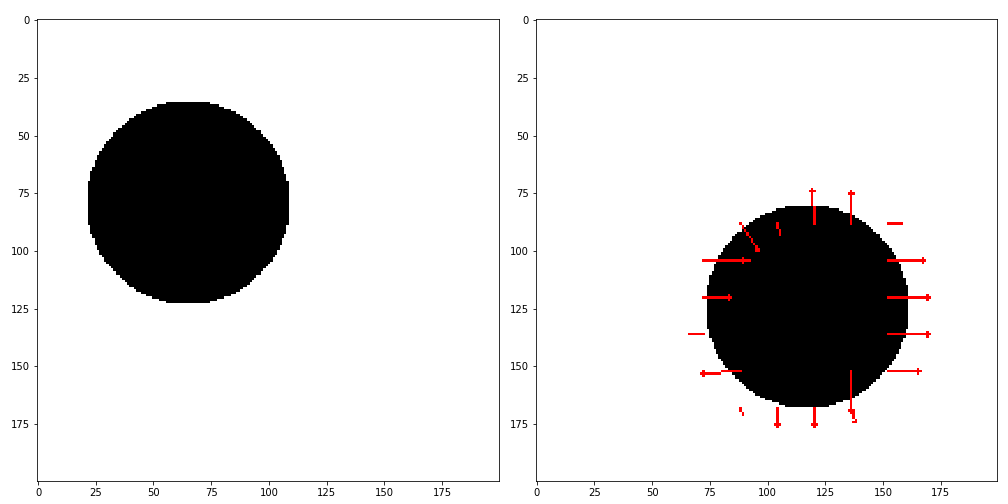
\includegraphics[width=\linewidth]{circle_diamond}
	\caption{Поиск векторов смещения при помощи ромбовидного поиска для монотонного изображения (0.03 секунды)}
\end{figure}

\begin{figure}[H]
	\centering
	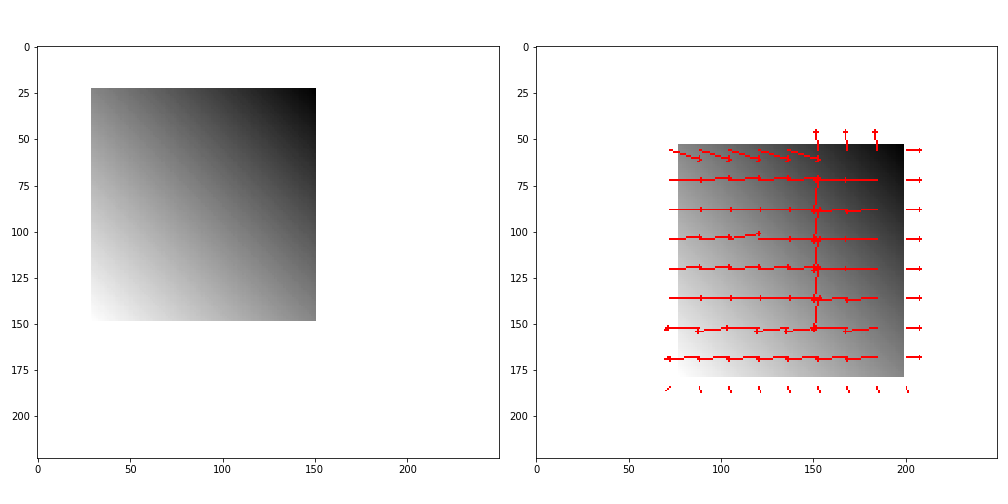
\includegraphics[width=\linewidth]{square_diamond}
	\caption{Поиск векторов смещения при помощи ромбовидного поиска для градиентного изображения (0.06 секунды)}
\end{figure}

Из результатов видно, что время работы алгоритма по сравнению с полным перебором меньше в несколько десятков раз. Тем не менее, алгоритм выдал менее точные результаты в примере с монотонным кругом.

\section{Выводы}

В данной работе были реализованы два алгоритма для поиска на изображении векторов смещения:

\begin{itemize}
	\item алгоритм полного перебора;
	\item алгоритм ромбовидного поиска.
\end{itemize}

Оба алгоритма успешно реализованы и протестированы на разных изображениях. Оба метода показали приемлемые результаты определения смещений, но скорость ромбовидного поиска оказалась в несколько раз выше, чем у полного перебора. Тем не менее, наиболее точные вектора смешения были определены при помощи полного перебора.

\end{document}
